\chapter{Word Embedding}
\label{ch:Capitulo 5}

\begin{quote}
  Este capítulo introduce el concepto de Word Embedding y describe de forma detallada el modelo desarrollado para este proyecto. 
\end{quote}

% PASADO A LA SECCIÓN DE REVISIÓN BIBLIOGRÁFICA
\section{Introducción a los Word Embeddings}
La comprensión del lenguaje natural a partir de datos textuales es una de las áreas más estudiadas dentro del ámbito de la Inteligencia Artificial. Esto se debe a la necesidad de una forma adecuada para la representación de información textual de manera que ésta pueda ser tratada de forma automática. En la literatura, se han abordado técnicas para resolver este problema bajo distintas perspectivas, las cuales se centran en obtener una representación de palabras o un conjunto de ellas (generalmente frases o párrafos), que nos permitan trabajar con la información que contienen. La forma más sencilla de representar información textual como vector es mediante \textit{one-hot embedding}, donde el mapeo de los datos textuales se realiza con un vector donde cada casilla se asocia al índice de cada palabra y contiene el número de veces que aparece dicha palabra en el texto. Sin embargo, esta representación resulta poco escalable y no funciona bien cuando se trabaja con vocabularios de gran tamaño, ni tampoco tiene en cuenta las relaciones que existen entre una palabra y las que le rodean (lo que resulta indispensable al trabajar con información textual). Este último problema es el que recogen las técnicas basadas en \textit{n-gramas}~\cite{jones2007representing}, las cuales intentan tener en cuenta, no sólo una palabra, sino también aquellas que se encuentran cercanas en el texto con el objetivo de modelar la información de manera más realista. Esta técnica no sólo ha sido aplicada a nivel de palabra, sino que también se han aplicado técnicas basadas en n-gramas a otros niveles, como puede ser al de frase o de carácter~\cite{wieting2016charagram}. Usar n-gramas conlleva la dificultad de determinar qué cantidad de información debe de ser la que se tenga en cuenta para una palabra en cuestión, ya que es difícil determinar (y sobretodo, generalizar) el tamaño de la ventana que se considera a cada lado del elemento a representar. Aun así, en las tareas que involucran Procesamiento de Lenguaje Natural, existen otras dificultades añadidas como pueden ser la ambigüedad del lenguaje, el tratamiento de anáforas o la posibilidad de trabajar con palabras que no se hayan contemplado a la hora de diseñar el modelo del lenguaje en cuestión~\cite{li2018word,anaphora}. Estos problemas han llevado al desarrollo de herramientas más sofisticadas como pueden ser los modelos con métodos basados en Modelo de Espacio Vectorial (VSM) o Asignación Latente de Dirichlet (LDA)~\cite{almeida2019word}. 

El concepto de Word Embedding se introduce con los Modelos de Lenguaje basados en Redes Neuronales (Neural Networks Language Model) basándose en la idea de que es más probable que dos palabras sean similares si se usan en contextos parecidos. La motivación detrás de esta idea reside en que dos palabras con un significado similar deben usarse de forma parecida, y por tanto, su representación debe de ser parecida también. Este tipo de modelos se caracterizan por ser modelos no supervisados, y algunos de las representaciones más conocidas son las unidades LSTM (Long-Short Term Memory), \textit{Redes Neuronales Recurrentes} (RNN) o \textit{Word2Vector}~\cite{li2018word}. El éxito de estos modelos se debe a los buenos resultados que se han obtenido al aplicarlos en problemas que requieran trabajar con información textual. Como consecuencia de ello, se utilizan en multitud de aplicaciones de diferentes campos de estudio y se ha destacado su eficacia respecto a otros métodos a la hora de trabajar con textos~\cite{indefense}. En nuestro caso, el objetivo es definir una representación que nos permita codificar alimentos procedentes de textos de recetas, para así identificar ingredientes y a su vez permitirnos detectar alimentos equivalentes (o incluso de uso equivalente). Este objetivo lo podemos lograr con modelos de Word Embedding puesto que tienen en cuenta el contexto que acompaña a las apariciones de cada palabra en el conjunto de entrenamiento de forma que se mantenga su significado en la codificación, a partir de cuándo, cómo y con qué otras palabras suele aparecer.
%El trabajar con las representaciones que se obtienen por medio de modelos de Word Embedding (las llamadas \textit{representaciones distribuidas}), nos permiten trabajar con codificaciones de palabras que tienen en cuenta la semántica a la hora de representar dicha palabra. Para ello, tienen en cuenta el contexto que acompaña a las apariciones de cada palabra en el conjunto de entrenamiento, de forma que se pueda mantener su significado en la codificación, a partir de cuándo, cómo y con qué otras palabras suele aparecer. 

Esta importancia del contexto a la hora de obtener la codificación de los datos textuales nos permitirá trabajar con los ingredientes de las recetas de manera más precisa, ya que, muchos de estos ingredientes serán similares (o su uso será parecido), o incluso se caracterizarán por poder nombrarse de más de una forma distinta. Como ejemplo de ello tenemos numerosos alimentos para los que se emplean más de un nombre de manera indistinta: sepia y choco, judías y habichuelas, pero y manzana, o incluso galleta y cookie. Además, por las características del lenguaje culinario, hay que tener en cuenta que las diferencias culturales y las marcas de alimentación se suelen ver involucradas con frecuencia en las recetas de cocina. Muchas veces se utiliza la marca del alimento en sustitución del propio alimento (p.ej., \textit{Danone} y yogur, pan \textit{Bimbo} y pan de molde), y otras veces, dependiendo del origen geográfico de la receta, un mismo alimento puede ser referido de distintas formas (p.ej., boniato y batata, melocotón y durazno, etc). El utilizar representaciones que sean capaces de tener en cuenta esta semántica (como es el caso de los modelos de Word Embedding) nos permitirá trabajar de una forma más adecuada con estos problemas y solventar dificultades procedentes del lenguaje como pueden ser las diferencias culturales mencionadas anteriormente, así como las asunciones de conocimiento que se hacen al hablar en términos de recetas y cocina en general. 
 
\section[Word embeddings generales vs específicos]{Word embeddings generales vs específicos en Food Computing}

Hoy en día, existen modelos de Word Embedding de carácter general ya entrenados sobre grandes cantidades de datos textuales procedentes de grandes bases de datos de documentos. Este es el caso, por ejemplo, del modelo Word2vec entrenado por Google\footnote{\url{https://code.google.com/archive/p/word2vec/}}, el cual incluye representaciones vectoriales de palabras para un vocabulario de 3 millones de palabras y frases entrenado a partir de 100 billones de palabras procedentes de un dataset de Google News. Estos modelos permiten abordar de manera eficaz con problemas de Procesamiento de Lenguaje Natural de manera superficial y sin profundizar en campos de conocimiento muy específicos. 

% mas modelos preentrenados aqui https://radimrehurek.com/gensim/auto_examples/howtos/run_downloader_api.html 

Sin embargo, en nuestro caso, al estar trabajando con un dominio tan específico como es el de la nutrición, surge la necesidad de utilizar modelos entrenados sobre dicho dominio concreto. Esto se debe principalmente a la gran cantidad de vocabulario especializado que es difícil de encontrar en un modelo de carácter general, y que limitaría la potencia de éste al no ser capaz de representar las descripciones alimenticias de manera correcta. A la hora de tratar con las descripciones textuales de los alimentos como si se tratasen de documentos cortos, cada una de las palabras pertenecientes al documento es representada usando el modelo de Word Embedding entrenado. Dado que el vocabulario del modelo no engloba todas las palabras de ese lenguaje, muchas de ellas no podrán representarse con este modelo. Estas palabras, denominadas \textit{out-of-vocabulary} (OOV)~\cite{8751687}, suponen un reto en las tareas de Procesamiento de Lenguaje Natural, y existen en la literatura múltiples formas de abordar este problema~\cite{camacho2018word}. Cuando una de estas palabras no tiene representación en el modelo, es omitida (o en algunos casos reemplazada), introduciendo ambigüedad en la representación final de dicho documento. 

En nuestro caso, donde gran parte del vocabulario referente a los alimentos es raramente usado fuera del contexto culinario o nutricional, el uso de un modelo de carácter general intensificaría el problema previamente comentado, dando lugar a representaciones muy precarias. Para ilustrar este problema, pongamos como ejemplo que queremos modelar la descripción alimenticia ``\textit{Tartaletas de escalibada con anchoas}". Teniendo en cuenta el tratamiento de las palabras OOV previamente comentado, supongamos que el modelo no capaz de detectar la palabra \textit{Tartaleta}, y por tanto ésta sea omitida a la hora de obtener la representación vectorial de dicha frase. De esta forma, dejaríamos de considerar la descripción original y pasaríamos a tener ``\textit{Escalibada con anchoas}". De igual forma podría pasar con \textit{Escalibada}, pasando a trabajar con ``\textit{Tartaletas de anchoas}", o incluso si no pudiéramos modelar ninguna de las dos palabras mencionadas, pasando a tener ''\textit{Anchoas}" (descripción que no se asemeja a la original). Con este ejemplo se pretende ilustrar que sin un modelo que tenga en cuenta de manera exhaustiva lenguaje alimenticio, no seríamos capaces de trabajar con representaciones precisas de descripciones de alimentos. Como consecuencia, no podríamos trabajar con los datos de una manera adecuada y fiable. 


De igual forma, tampoco podríamos trabajar de manera precisa con el vocabulario de un modelo genérico de Word Embedding. Por ejemplo, al intentar obtener las palabras más similares del vocabulario, en un modelo genérico no obtendríamos el nivel de exactitud que podríamos conseguir con un modelo generado a partir de contenido específico. Ejemplo de ello se muestra en la Tabla \ref{table1}, donde se muestran los resultados de alimentos más parecidos a uno previamente proporcionado obtenidos con un Word Embedding de propósito general y con uno específico de alimentación (ver columnas \textit{Alimento}). De igual forma, en la Tabla \ref{table1}, podemos ver en las columnas \textit{Similitud} el grado de similitud (cuyo valor se encuentra entre 0 y 1, siendo 1 la similitud máxima entre dos elementos) de los alimentos más similares obtenidos por cada modelo de Word Embedding. En los resultados expuestos en dicha tabla, se observa cómo para una misma palabra (en este caso \textit{ajo}) se obtienen resultados más cercanos a la palabra original con el modelo correspondiente a un Word Embedding especializado en alimentación. En el Capítulo \ref{ch:Pruebas} (Sección \ref{WordEmbedding}) se muestra una comparativa del uso de Word Embedding específico y genérico en este problema que corrobora estas afirmaciones.

\setlength{\tabcolsep}{10pt} 
\begin{table}[h]
\caption{\label{table1}Similitudes para \textit{ajo} con modelos de W.E.}
\centering
\begin{tabular}{cccc}
\hline
\multicolumn{2}{c}{\textbf{W.E. (General)}} & \multicolumn{2}{c}{\textbf{W.E. (Específico)}} \\ \hline
 \textbf{Alimento} & \textbf{Similitud} & \textbf{Alimento} & \textbf{Similitud} \\ \hline \hline
hinojo & 0.7304 &  diente de ajo & 0.5661 \\ \hline
orégano & 0.7030 &  cebolla & 0.5097 \\ \hline
perejil & 0.7022 &  chalota & 0.4825 \\ \hline
laurel & 0.6971 & ajo en polvo& 0.4796 \\ \hline
cilantro & 0.6914 & cúrcuma & 0.4525 \\ \hline
cebolla & 0.6913 &  comino & 0.4479 \\ \hline
\end{tabular}
\end{table}
% para justificar la omisión de las OOV, que Word document distance lo hace, y que al final en los alimentos es relativamente facil englobar todo el vocabulario a través de las recetas y no muchas palabras se van a quedar fuera. 

Por último, es importante tener en cuenta la naturaleza del dominio en el que estamos trabajando, donde las recetas y los textos relativos a la alimentación suelen mantener un vocabulario \textit{cerrado}. Con ello nos referimos a que, suelen utilizarse siempre los mismos verbos (o sinónimos de los mismos), y que las recetas suelen utilizar en su mayor parte un gran número de ingredientes comunes. Con ello, pretendemos ilustrar que, con una gran cantidad de recetas, podríamos obtener de forma sencilla una muestra representativa de los diferentes alimentos que se ven involucrados en la cocina. 

Por esta facilidad a la hora de modelar el vocabulario involucrado en el mundo culinario, así como por todas las otras razones previamente expuestas, se ha decidido utilizar un modelo de Word Embedding entrenado de manera específica sobre datos textuales procedentes de repositorios relacionados con el mundo de la alimentación, para así poder trabajar con su vocabulario de la forma más exhaustiva posible. 

\section{Metodología}

Para abordar el diseño e implementación del modelo de Word Embedding, se han distinguido cuatro pasos principales, explicados a lo largo de este capítulo. En primer lugar definiremos los datos utilizados y la propia creación del corpus para el entrenamiento del modelo (Subsección \ref{subsec:datos}), el preprocesamiento llevado a cabo a dichos datos (Subsección \ref{subsec:preprocessing}) y la implementación y entrenamiento del modelo (Subsección \ref{subsec:implementacion} y Subsección \ref{subsec:train} respectivamente).

\subsection{Datos utilizados}\label{subsec:datos}

Se ha decidido utilizar como conjunto de entrenamiento una colección de textos de preparación de recetas en inglés para entrenar el modelo de Word Embedding. Esta decisión ha venido condicionada por la gran cantidad de contenido de esta naturaleza que se puede encontrar en Internet, así como por la existencia de grandes repositorios de recetas cuyos datos contienen información textual que podemos procesar. 

En este tipo de textos podemos encontrar los ingredientes de las recetas así como el uso que se le da a estos, con qué tipo de verbos se combinan, con qué ingredientes se mezclan, y una gran cantidad de información intrínseca que puede facilitar la representación de un ingrediente, así como la identificación del mismo a posteriori. Esto se debe a que gracias a la información que se encuentra en los textos de preparación de las recetas, podríamos identificar otros ingredientes con el mismo comportamiento, que aparezcan junto a los mismos ingredientes, o se utilicen los mismos verbos. Esta funcionalidad da lugar a múltiples aplicaciones que pueden ser aplicadas sobre los ingredientes, como la identificación de ingredientes sustitutos o equivalentes (por ejemplo, ``\textit{Tartaleta}`` y ``\textit{Pasta de hojaldre}") .

En un principio vamos a trabajar con recetas cuyo texto se encuentra en inglés. Las razones de esta decisión son las siguientes: 

\begin{itemize}
    \item La mayor parte de los repositorios disponibles de recetas trabajan con textos de preparación e ingredientes en inglés. 
    
    \item Las bases de datos de referencia de composición nutricional de alimentos está en inglés. Por otra parte, las bases de datos cuyo idioma original difiere del inglés, incluyen traducciones de los campos textuales a éste, lo que nos permitiría trabajar con dichas bases de datos de igual forma. 
    
    \item Debido a la internacionalización de las recetas, disponemos de una amplia selección de recetas en inglés que cubren las distintas culturas culinarias independientemente de la región geográfica de las que provengan. De esta forma, podremos trabajar en inglés con recetas de todo el mundo, sin encontrar restricciones de idioma. 
\end{itemize}

Esta decisión tiene como consecuencia que el modelo entrenado nos obligará a trabajar con contenido en inglés. Sin embargo, tal y como se ha expuesto en los puntos anteriores, gracias a la internacionalización de las recetas que existe hoy en día, no tendremos problemas referentes a restricciones en cuanto al contenido de las mismas, sino que de esta forma podremos trabajar en nutrición de forma internacional sin centrarnos en países concretos. 

\begin{table}[H]
\centering
\caption{\label{table2}Ejemplo de receta: Noodles en 5 minutos}

\begin{tabular}{m{11.5cm}}
\hline
\multicolumn{1}{c}{\textbf{5 minutes noodles}} \\ \hline \hline
Pour 700ml freshly \textbf{boiled} water into a saucepan, add the stock cube and \textbf{stir} well to \textbf{dissolve}. Add the noodles, spring onions, peas and chicken, \textbf{bring} to the boil and \textbf{cook} for 5 minutes, or until the noodles and peas are \textbf{cooked} and the chicken is hot through. \\ \hline %Ladle into a deep, wide bowl and, if you fancy, top with the chilli, ginger, garlic, coriander and soy.
\end{tabular}
\end{table}

En la Tabla \ref{table2} se muestra un ejemplo de las recetas que utilizaremos para entrenar el modelo de Word Embedding. En ella, se han señalado los verbos típicos que encontraremos en este tipo de recetas, como muestra del vocabulario tan concreto (y también cerrado, sobretodo en el caso de los verbos) con el que estaremos trabajando.
 
Para formar el corpus de recetas con el que entrenaremos el modelo de Word Embedding hemos utilizado una colección de recetas publicada por archive.org\footnote{\url{https://archive.org/download/recipes-en-201706}}. En esta colección se encuentran recopiladas un total de 267,071 recetas correspondientes a los sitios web enumerados a continuación (la distribución de recetas según sitio web se puede observar en la Tabla \ref{table3}).

\begin{itemize}
    \item \textit{AllRecipes.com}{\footnote{Sitio web de AllRecipes: \url{https://www.allrecipes.com/}}}: red social centrada en el mundo de cocina en la que se puede compartir y encontrar recetas, trucos de cocina, fotos y vídeos con el objetivo de inspirar a usuarios para crear nuevas recetas. Su página de recetas es una de las más visitadas del mundo. 
    \item \textit{BBC Food Recipe}{\footnote{Sitio web de BBC Recipes: \url{https://www.bbc.co.uk/food/recipes}}}: colección de recetas procedentes de los programas y chefs de la BBC, la principal emisora de servicio público del mundo. En ella se pueden encontrar recetas clasificadas por estación, festividades, e incluso por ingredientes. 
    \item \textit{Epicurious}{\footnote{Sitio web de Epicurious: \url{https://www.epicurious.com/}}}: es una marca digital para consumidores centrada en la comida y el arte culinario. Tiene más de 300,000 recetas, así como vídeos y recetas y consejos para la cocina del día a día.
    \item \textit{CookStr}{\footnote{Sitio web de CookStr: \url{https://www.cookstr.com/}}}: sitio web de recetas cuyo objetivo se centra en organizar los libros de cocina de éxito así como las recetas del mundo y hacerlos universalmente accesibles.
\end{itemize}

\begin{table}[H]
\centering
\begin{center}
    {\caption{Corpus de recetas: origen y número de recetas} \label{table3}}
    \begin{tabular}{cc}
        \hline
        \textbf{Procedencia} & \textbf{Número de recetas} \\ \hline \hline
        BBC Food Recipe & 10,679 \\ \hline
        Epicurious & 20,111 \\ \hline
        Cookstr & 225,602 \\ \hline
        AllRecipes & 10,679 \\ \hline \hline
        \textbf{Total de recetas} & \textbf{267,071} \\ \hline
        \end{tabular}
\end{center}
\end{table}

Dicha colección se distribuye en ficheros de extensión .json clasificados por el sitio web de procedencia de la receta. De esta forma, disponemos de cuatro ficheros con recetas, donde cada uno de ellos está formado por la lista total de recetas obtenidas de dicho sitio web. En la Figura \ref{fig:estructura-recetas} se muestra la estructura de las recetas que forman este repositorio. 

\begin{figure}[H]
    \centering
    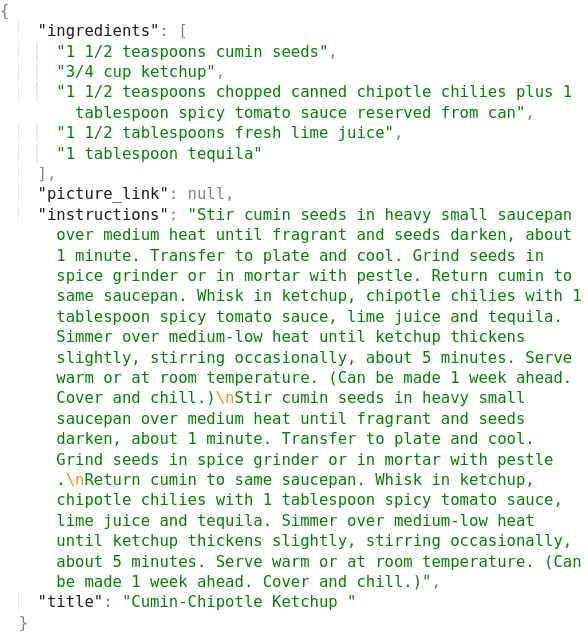
\includegraphics[width=0.75\textwidth]{imagenes/ejemplo-json-2.png}
    \caption{Estructura de las recetas en el dataset de archive.org}
    \label{fig:estructura-recetas}
\end{figure}

\subsection{Preprocesamiento de los datos textuales}\label{subsec:preprocessing}

Como se puede apreciar en la Figura \ref{fig:estructura-recetas}, los datos textuales de las recetas no se encuentran en un formato directamente manipulable para entrenar un modelo de lenguaje. Por ello, es necesario aplicar técnicas de preprocesamiento de datos que permitan su limpieza y adecuación para poder ser usados como datos de entrada en el entrenamiento del modelo de Word Embedding. En este paso, así como en todo el proceso de creación del modelo, haremos uso de la librería de Topic Modelling  Gensim\footnote{\url{https://radimrehurek.com/gensim/}}. Esta librería de código abierto proporciona funciones para trabajar con problemas de Procesamiento de Lenguaje Natural en el lenguaje de programación Python, y en particular, para entrenar y trabajar con modelos de Word Embedding. Con las funciones implementadas en dicha librería, podremos tanto entrenar como utilizar con facilidad el modelo, así como llevar a cabo las tareas de limpieza y preprocesamiento de los datos que utilicemos.

\subsubsection{Creación del corpus}

En primer lugar, hay que crear un corpus que recoja todos los datos textuales con los que se va a trabajar. Como ya se ha mencionado en secciones previas, los datos se encuentran distribuidos en cuatro ficheros, cada uno de ellos con una lista de las recetas obtenidas de los sitios web de recetas previamente mencionados. Por tanto, se requiere un preprocesamiento previo de cada uno de los ficheros correspondientes de forma que podamos disponer de una sola colección de datos que contenga únicamente la información textual que vamos a utilizar. Dicho de otra forma, debemos reestructurar la información para poder trabajar con un corpus con todos los datos textuales procedentes de los textos de preparación de las recetas que tenemos. 

Para solventar esta dificultad, se ha generado un fichero por cada receta con el texto de su preparación, de forma que únicamente trabajemos con ficheros cuyos datos son los que nos interesa preprocesar. De manera automatizada, se lee cada uno de los ficheros previamente generados para formar el corpus de recetas. En la Figura \ref{fig:creacion-corpus} se aprecia de forma esquematizada el procedimiento para montar este corpus.

\begin{figure}[H]
    \centering
  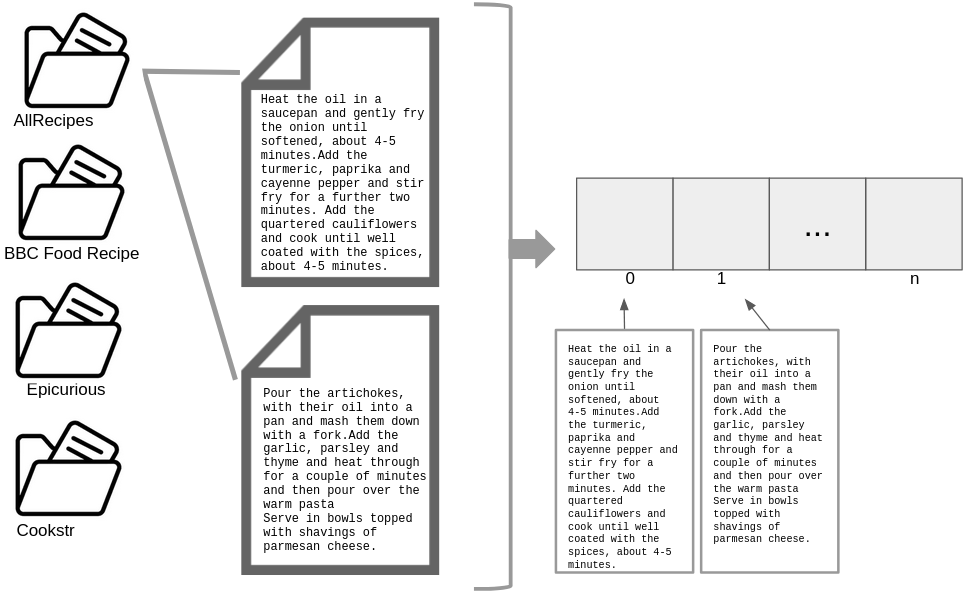
\includegraphics[width=0.8\textwidth]{imagenes/creacion-corpus-gris.png}
  \caption{Procedimiento para formar el corpus de recetas}
  \label{fig:creacion-corpus}
\end{figure}


\subsubsection{Limpieza del corpus}

Como se ha podido observar en ejemplos previos, el texto de preparación de las recetas se encuentra sin ningún tipo de procesamiento previo, y por ello necesita un tratamiento adecuado de la información textual para que el modelo de Word Embedding proporcione resultados de calidad. En nuestro caso, para el mencionado corpus de recetas se ha llevado a cabo la limpieza y tokenización que se presenta a continuación. Para complementar los pasos, utilizaremos como ejemplo el siguiente texto de preparación que se corresponde con una de las recetas del dataset: ``\texttt{Combine Ranch, salsa, tomatoes and chilies, if desired. Chill 1 hour. Serve with tortilla chips.}"

\begin{enumerate}
    
    \item \textbf{Tokenización del texto}. Se obtienen los tokens del fichero. Al generar los tokens se lleva a cabo la eliminación de símbolos (incluidos los de puntuación), dígitos, y pasar texto a minúsculas. Como resultado, se obtiene el texto como una lista de tokens con las palabras del fichero formadas por caracteres alfabéticos. Tras aplicar estos cambios, el ejemplo quedaría de la siguiente manera:
    
    \begin{center}
    
        \texttt{[`combine', `ranch', `salsa', `tomatoes', `and', `chilies', `if', `desired', `chill', `hour', `serve', `with', `tortilla', `chips']}
        
    \end{center}
    
    
    \item \textbf{Eliminación de las llamadas \textit{stopwords}}. Las stopwords son palabras muy comunes del vocabulario, que no van a proporcionar información útil, y por tanto es recomendable prescindir de ellas~\cite{saif2014stopwords}. Ejemplos de stopwords en inglés pueden ser ``the", ``a", ``my", ``your", etc. Para este caso, hemos utilizado la lista de stopwords en inglés proporcionada por la librería \textit{Gensim}. En este punto, el fichero tomado como ejemplo quedaría como se muestra a continuación:
    
    \begin{center}
        \texttt{[`combine', `ranch', `salsa', `tomatoes', `chilies', `desired', `chill', `hour', `serve', `tortilla', `chips']}
    \end{center}
    
    En el ejemplo se aprecia cómo se han eliminado aquellas palabras incluidas en el vocabulario de stopwords (en este caso, las stopwords existentes en el ejemplo son `\texttt{the}', `\texttt{if}'  y `\texttt{with}').\\
    

    \item \textbf{Aplicación de lematización}. Por último, aplicaremos una normalización lingüística al corpus conocida como lematización. Mediante esta técnica, se reducen todas las palabras a su raíz, de forma que se transforman las distintas variaciones morfológicas de una palabra a una única forma común. Esto ocurrirá, por ejemplo, con los verbos, donde nos encontraremos un mismo verbo en sus distintas formas verbales cuando todos ellos hacen referencia a una misma acción (así forzaremos a tener una única forma de aparición de los mismos). Tras aplicar la normalización comentada, el fichero quedaría de la siguiente forma:
    
    \begin{center}
        \texttt{[`combin', `ranch', `salsa', `tomato', `chili', `desir', `chill',  `hour', `serv', `tortilla', `chip']}
    \end{center}
    
    En dicho ejemplo se puede observar el caso comentado sobre los verbos, los cuales se han llevado a su raíz (como ocurre en el caso de `\texttt{serve}', que pasa a ser `\texttt{serv}'). También podemos ver que como resultado de dicha normalización se ha eliminado el plural de las palabras (`\texttt{tomatoes}' pasa a ser `\texttt{tomato}'). 
\end{enumerate}

\subsubsection{Detección de bigramas}
Por otra parte, en el lenguaje natural es normal que aparezcan palabras compuestas. El lenguaje culinario no es una excepción, y también existen palabras que suelen aparecer siempre juntas, como puede ser ``\textit{pimienta negra}", ``\textit{vino tinto}" o ``\textit{azúcar moreno}". Este tipo de casos, donde hay palabras que tienen más sentido ser tratadas como una sola que de manera independiente, da lugar al uso de técnicas de bigramas, que permiten tratar palabras (o en nuestro caso, tokens) de manera colectiva como si de una única se tratase. 

Para llevar esta idea a la práctica, en primer lugar es necesario entrenar el modelo de bigramas a partir de todos los textos que forman el corpus, para así poder detectar qué palabras son las que aparecen juntas una cantidad de veces considerable y poder representarlas en el texto como si fueran una sola. Esto se lleva a cabo sobre los datos una vez limpiados de la forma descrita en la sección anterior. Para este paso, también se ha hecho uso de las utilidades propocionadas por la librería Gensim. 

Una vez entrenado el modelo de bigramas, éste es aplicado sobre el mismo corpus para sustituir aquellos tokens de los que se detecten bigramas. A continuación se muestra cómo quedaría el ejemplo utilizado en el apartado anterior tras la detección de bigramas.

\begin{center}
    \texttt{[`combin', `ranch', `salsa', `tomato', `chili', `desir', `chill', `hour', `serv', `tortilla\_chip']}
\end{center}

Tal y como se puede ver, los token `\texttt{tortilla}' y `\texttt{chip}' pasarían a ser un token único (`\texttt{tortilla\_chip}'), lo cual es de esperar porque son dos palabras que, en las recetas, suelen encontrarse siempre juntas ya que se trata de un alimento cuya descripción textual es una palabra compuesta. 


\subsection{Implementación de Word2vec}\label{subsec:implementacion}
Para construir el modelo lingüístico a partir del corpus de recetas descrito en las secciones anteriores se pueden utilizar distintos algoritmos no supervisados estandarizados. Entre los más conocidos, se encuentran Word2Vec~\cite{mikolov2013distributed, mikolov2013efficient}, Glove~\cite{pennington2014glove} o fasttext~\cite{bojanowski2016enriching}. 
En este trabajo, se ha optado por utilizar el algoritmo Word2vec para entrenar el Word Embedding. De este algoritmo existen diferentes implementaciones; las más conocidas son las denominadas \textit{Continuous Bag of Words} and \textit{Skip-Gram} \cite{rong2014word2vec}. A continuación, se explica de forma detallada en qué consisten estas implementaciones. 

\subsubsection{Modelo Continuous Bag of Words (CBOW)}
Esta implementación de Word2vec se centra en predecir una palabra a partir del contexto, cuya estructura puede apreciarse en la Figura \ref{fig:cbow-1}. La capa de entrada de la red ($X$) representará el contexto, la capa oculta ($H)$ hace referencia al Embedding entrenado y la capa salida ($Y$) representará la palabra de la que se quiere obtener su representación en el modelo. Este contexto puede estar formado por una o más palabras. En el caso de que el contexto esté formado por una única palabra, estaríamos en la versión simplificada de este modelo (que es la mostrada en la Figura \ref{fig:cbow-1}). Independientemente del tamaño tenido en cuenta en el contexto, cada una de las palabras que formen parte del mismo se encuentran codificadas mediante el método \textit{one-hot-enconding} explicado en secciones anteriores. Este vector tendrá como tamaño el del vocabulario (notado por $V$), y estará completo a valor 0 exceptuando las posiciones que se correspondan con la palabra (o palabras) que se utilicen en el contexto, cuyo valor será 1.

% enos uno de sus elementos, cuyo valor será 1. Este elemento será el correspondiente a la palabra del vocabulario que coincida con la palabra del contexto que se quiera codificar en ese momento. Dicho de otra forma, la codificación de una palabra del contexto identificada en el vocabulario del modelo como $v_i$, se codificará como el vector $X$, de tamaño $V$. Dicho vector $X$ tendrá valor 0 en todos sus elementos, a excepción del elemento $X_i$ el cual tendrá valor 1.
    
\begin{figure}[H]
    \centering
    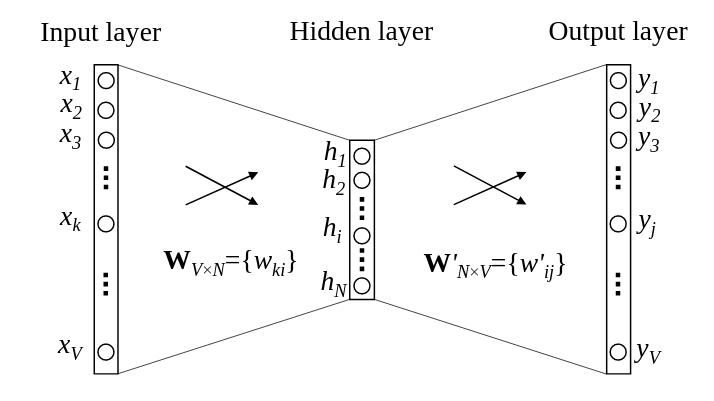
\includegraphics[width=0.65\textwidth]{imagenes/cbow_esquema.png}
    \caption{Modelo CBOW donde el contexto es una palabra~\cite{rong2014word2vec}}
  \label{fig:cbow-1}
\end{figure}
    
\subsubsection{Modelo Skip-Gram}
En este modelo, se lleva a cabo el procedimiento inverso. A pesar de que la capa oculta ($H$) sigue representando el Embedding, en este caso, la capa de entrada del modelo ($X$) es la palabra que corresponde a la capa de salida en el modelo CBOW (es decir, el target). Tal y como se puede ver en la Figura \ref{fig:modelos-w2v}b, la capa de salida ($Y$) de este modelo está formada por el contexto correspondiente a la palabra proporcionada como entrada. En otras palabras, mientras que en el modelo CBOW lo que se predice es la palabra, en el modelo Skip-Gram lo que se pretende predecir es el contexto de dicha palabra. En la selección de Figuras \ref{fig:modelos-w2v} se puede ver de forma gráfica esta diferencia existente entre los modelos. 

\begin{figure}[h!]
    \centering
    \begin{subfigure}[b]{0.47\textwidth}
        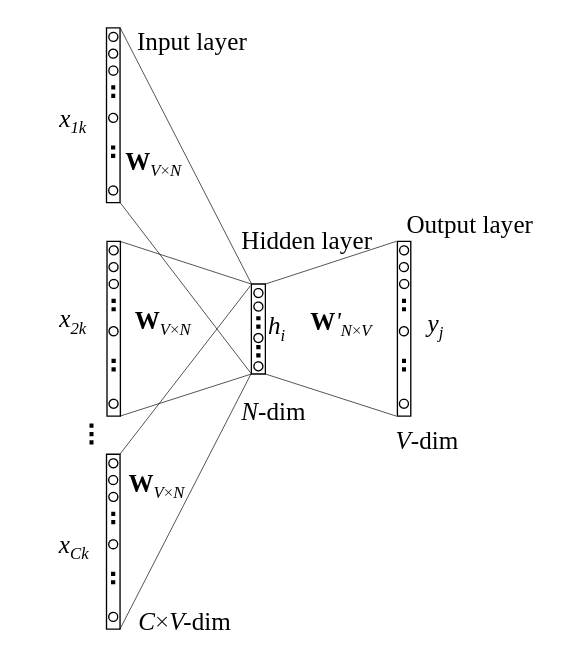
\includegraphics[width=1.0\textwidth]{imagenes/cbow_esquema2.png}
        \caption{Modelo CBOW}
    \end{subfigure}
    \begin{subfigure}[b]{0.47\textwidth}
        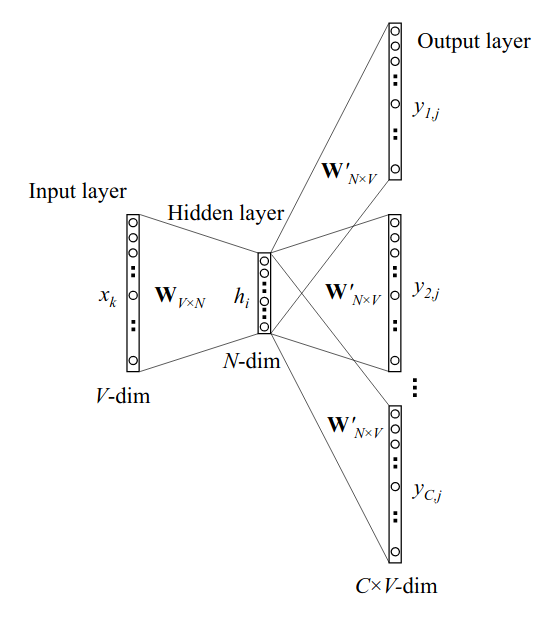
\includegraphics[width=1.0\textwidth]{imagenes/skipgram_esquema.png}
        \caption{Modelo Skip-gram.}
    \end{subfigure}
    \caption{Modelos del algoritmo Word2vec~\cite{rong2014word2vec}}
    \label{fig:modelos-w2v}
\end{figure}


Como es de esperar, ambos modelos tienen sus ventajas y desventajas, y cada uno de ellos es más o menos apropiado en función del problema en cuestión. En líneas generales, el modelo CBOW suele funcionar mejor con palabras del vocabulario que aparecen con frecuencia, mientras que Skip-Gram es capaz de obtener buenas representaciones para vocabulario poco frecuente en el corpus utilizado para entrenar el modelo de Word Embedding. 

\subsection{Entrenamiento del modelo}\label{subsec:train}
Para el entrenamiento del modelo de Word Embedding a partir del corpus de recetas hemos decidido utilizar la implementación de Word2vec \textit{Continuous Bag of Words} (CBOW). La razón principal reside en su implementación, que permite obtener buenas representaciones para palabras de uso frecuente. Esto es especialmente adecuado para nuestro problema dado que en el vocabulario culinario hay una gran cantidad de palabras que aparecen con mucha frecuencia en los textos. Al igual que con la creación del corpus y su preprocesamiento, hemos utilizado las funcionalidades de la librería Gensim para llevar a cabo el entrenamiento del modelo. En el Capítulo \ref{ch:Pruebas} se detalla la experimentación y el ajuste de hiperparámetros realizado.